\subsection{Módulo de Visualización y Gemelo Digital (VIS)}

\begin{figure}[H]\centering
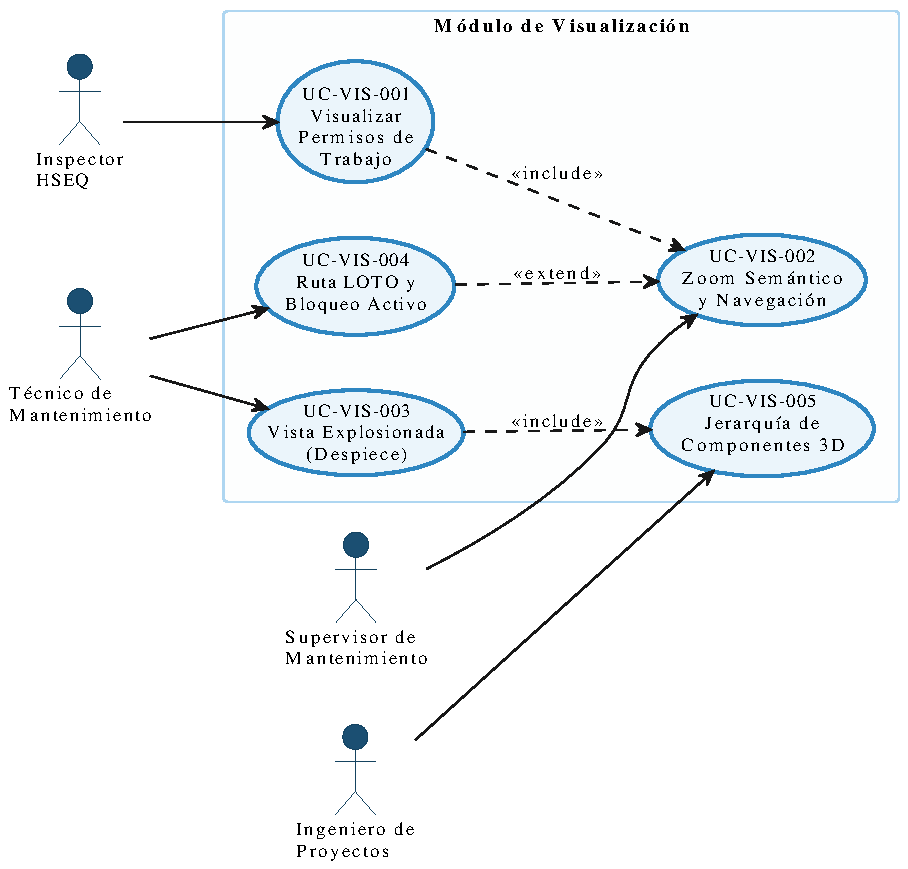
\includegraphics[width=0.85\textwidth]{assets/Diagrama-UC-VIS.pdf}
\caption{Diagrama de Casos de Uso - Visualización y Gemelo Digital}\end{figure}

\noindent\textbf{Ficha de Caso de Uso: UC-VIS-004 - Visualización de Rutas de Aislamiento (LOTO) y Bloqueo Activo}
\footnotesize\setlength{\tabcolsep}{4pt}\renewcommand{\arraystretch}{1.2}
\rowcolors{2}{tableBlue}{white}\begin{longtable}{>{\raggedright\arraybackslash}p{0.21\textwidth} >{\raggedright\arraybackslash}p{0.74\textwidth}} \toprule
\textbf{Actor Principal} & Técnico de Mantenimiento \\
\textbf{Actores Secundarios} & Supervisor HSEQ (notificado), Ingeniero de Seguridad (valida) \\
\textbf{Descripción} & Permite visualizar rutas de aislamiento de energía y aplicar bloqueo activo para garantizar condiciones de Energía Cero antes de iniciar una intervención. \\
\textbf{Precondiciones} & \parbox[t]{\linewidth}{\vspace{2pt} \begin{itemize}[leftmargin=1.5em, nosep, topsep=0pt]
\item La OT requiere LOTO y está asignada al Técnico
\item Los puntos de aislamiento están definidos para el activo
\item El Técnico está autenticado y autorizado [TR-006]
\end{itemize} \vspace{2pt}} \\
\textbf{Flujo Principal} & \parbox[t]{\linewidth}{\vspace{2pt} \begin{enumerate}[leftmargin=1.5em, nosep, topsep=0pt]
\item El Técnico abre la OT y selecciona ``Ver Ruta LOTO'' (FR-225).
\item El Sistema activa el estado de aislamiento LOTO y presenta la ruta de aislamiento con puntos críticos (FR-226, FR-227).
\item El Sistema presenta la lista de verificación ``Checklist LOTO'' con los puntos a confirmar (FR-228).
\item El Sistema valida el estado de energía y mantiene bloqueado el inicio del trabajo si detecta energía activa (FR-229).
\item El Técnico confirma físicamente cada punto de aislamiento en la lista (FR-228, FR-230).
\item El Sistema solicita confirmación final y registra la validación de aislamiento (FR-230, [TR-001]).
\item El Sistema habilita la función ``Iniciar Trabajo'' (FR-231).
\item El Técnico inicia la ejecución y el Sistema cambia la OT a ``En Ejecución'' con auditoría (FR-231, [TR-001]).
\end{enumerate} \vspace{2pt}} \\
\textbf{Flujos Alternativos} & \parbox[t]{\linewidth}{\vspace{2pt} \vspace{4pt}\noindent\textbf{AF-001: Energía Activa Detectada}
\newline
En el paso 4, si se detecta energía activa:
\begin{enumerate}[leftmargin=1.5em, nosep, topsep=0pt]
\item El Sistema bloquea el inicio y notifica alerta crítica (FR-229).
\item El flujo regresa al paso 3.
\end{enumerate}
\vspace{4pt}\noindent\textbf{AF-002: Confirmación Incompleta}
\newline
En el paso 5, si no se confirman todos los puntos:
\begin{enumerate}[leftmargin=1.5em, nosep, topsep=0pt]
\item El Sistema mantiene el bloqueo de inicio (FR-230).
\item El flujo regresa al paso 3.
\end{enumerate}
\vspace{4pt}\noindent\textbf{AF-003: Reaparición de Energía Durante la Ejecución}
\newline
Después del paso 8, si se detecta energía activa:
\begin{enumerate}[leftmargin=1.5em, nosep, topsep=0pt]
\item El Sistema genera alerta inmediata y suspende la OT (FR-232).
\item Notifica al Supervisor HSEQ.
\end{enumerate} \vspace{2pt}} \\
\textbf{Postcondiciones} & \parbox[t]{\linewidth}{\vspace{2pt} \begin{itemize}[leftmargin=1.5em, nosep, topsep=0pt]
\item El trabajo inicia únicamente bajo condición de Energía Cero
\item El evento queda auditado de forma inmutable [TR-001]
\item El Supervisor HSEQ recibe notificación ante riesgo crítico
\end{itemize} \vspace{2pt}} \\
\textbf{Requisitos} & FR-225 a FR-232 [TR-001, TR-006, TR-007, TR-010, TR-011] \\ \bottomrule
\end{longtable}\normalsize\vspace{1em}
\noindent\textbf{Ficha de Caso de Uso: UC-VIS-001 - Visualización de Capa de Permisos de Trabajo}
\footnotesize\setlength{\tabcolsep}{4pt}\renewcommand{\arraystretch}{1.2}
\rowcolors{2}{tableBlue}{white}\begin{longtable}{>{\raggedright\arraybackslash}p{0.21\textwidth} >{\raggedright\arraybackslash}p{0.74\textwidth}} \toprule
\textbf{Actor Principal} & Inspector HSEQ \\
\textbf{Actores Secundarios} & Supervisores HSEQ, Contratistas (consultados) \\
\textbf{Descripción} & Permite visualizar permisos de trabajo activos sobre el mapa de planta con codificación visual estandarizada y validación de integridad. \\
\textbf{Precondiciones} & \parbox[t]{\linewidth}{\vspace{2pt} \begin{itemize}[leftmargin=1.5em, nosep, topsep=0pt]
\item El Inspector está autenticado con rol HSEQ [TR-006]
\item Existe información vigente de permisos de trabajo
\item El modelo de planta está cargado
\end{itemize} \vspace{2pt}} \\
\textbf{Flujo Principal} & \parbox[t]{\linewidth}{\vspace{2pt} \begin{enumerate}[leftmargin=1.5em, nosep, topsep=0pt]
\item El Inspector activa la capa ``Permisos de Trabajo'' (FR-182).
\item El Sistema presenta indicadores visuales de permisos con codificación visual estandarizada (FR-183).
\item El Inspector selecciona un permiso y el Sistema presenta información resumida con detalles (FR-184).
\item El Sistema valida integridad de referencias y detecta enlaces rotos (FR-185, [TR-003]).
\item Si hay permisos sin correspondencia, el Sistema presenta la sección de ``Incidencias de Visualización'' (FR-186).
\item El Inspector filtra permisos por tipo cuando es necesario (FR-188).
\item El Sistema registra la activación de capa, filtros y correcciones (FR-189, [TR-001]).
\end{enumerate} \vspace{2pt}} \\
\textbf{Flujos Alternativos} & \parbox[t]{\linewidth}{\vspace{2pt} \vspace{4pt}\noindent\textbf{AF-001: Fuente de datos no disponible}
\newline
En el paso 1, si la fuente de permisos no responde:
\begin{enumerate}[leftmargin=1.5em, nosep, topsep=0pt]
\item El Sistema notifica alerta y conserva el último estado confiable (FR-187).
\item El flujo regresa al paso 1.
\end{enumerate}
\vspace{4pt}\noindent\textbf{AF-002: Enlace roto detectado}
\newline
En el paso 4, si existe permiso sin correspondencia:
\begin{enumerate}[leftmargin=1.5em, nosep, topsep=0pt]
\item El Sistema notifica alerta de integridad y registra el permiso en incidencias (FR-185, FR-186).
\item El flujo continúa en el paso 5.
\end{enumerate} \vspace{2pt}} \\
\textbf{Postcondiciones} & \parbox[t]{\linewidth}{\vspace{2pt} \begin{itemize}[leftmargin=1.5em, nosep, topsep=0pt]
\item La capa de permisos queda visible con información vigente
\item Los eventos críticos quedan auditados [TR-001]
\item Los permisos sin correspondencia quedan identificados para corrección
\end{itemize} \vspace{2pt}} \\
\textbf{Requisitos} & FR-182 a FR-189 [TR-001, TR-003, TR-006, TR-010, TR-011] \\ \bottomrule
\end{longtable}\normalsize\vspace{1em}